\documentclass[12pt]{article}
\usepackage[utf8]{inputenc}
\usepackage[top=0.75in, bottom=0.75in, left=0.75in, right=0.75in, headheight=15pt]{geometry}
\usepackage{amsmath, amssymb, amsthm, graphicx, hyperref, enumerate, multirow,  multicol, tikz, centernot, cancel, forest, lipsum, mathtools, bm, esvect, fancyhdr, esdiff, float, parskip, comment}

\DeclareMathSymbol{*}{\mathbin}{symbols}{"01} % change * to /cdot inside math
% \begingroup % let only this align, etc. break across pages
% \allowdisplaybreaks
% \begin{align}
%     ....
% \end{align}
% \endgroup

% \begin{figure}[H]
%     \centering
%     \includegraphics{}
%     \caption{}
%     \label{fig:}
% \end{figure}

% \texorpdfstring{$k$}{k} math inside (sub/)section label

\pagestyle{fancy}
\fancyhead[L]{Liheng Cao}
% \fancyhead[C]{center}
\fancyhead[R]{}

\title{} % title
\author{Liheng Cao} % name
\date{\today} % custom date else today's date

\begin{document}
\maketitle

\section{}
\begin{enumerate}[(a)]
	\item \, \begin{figure}[H]
		\centering
		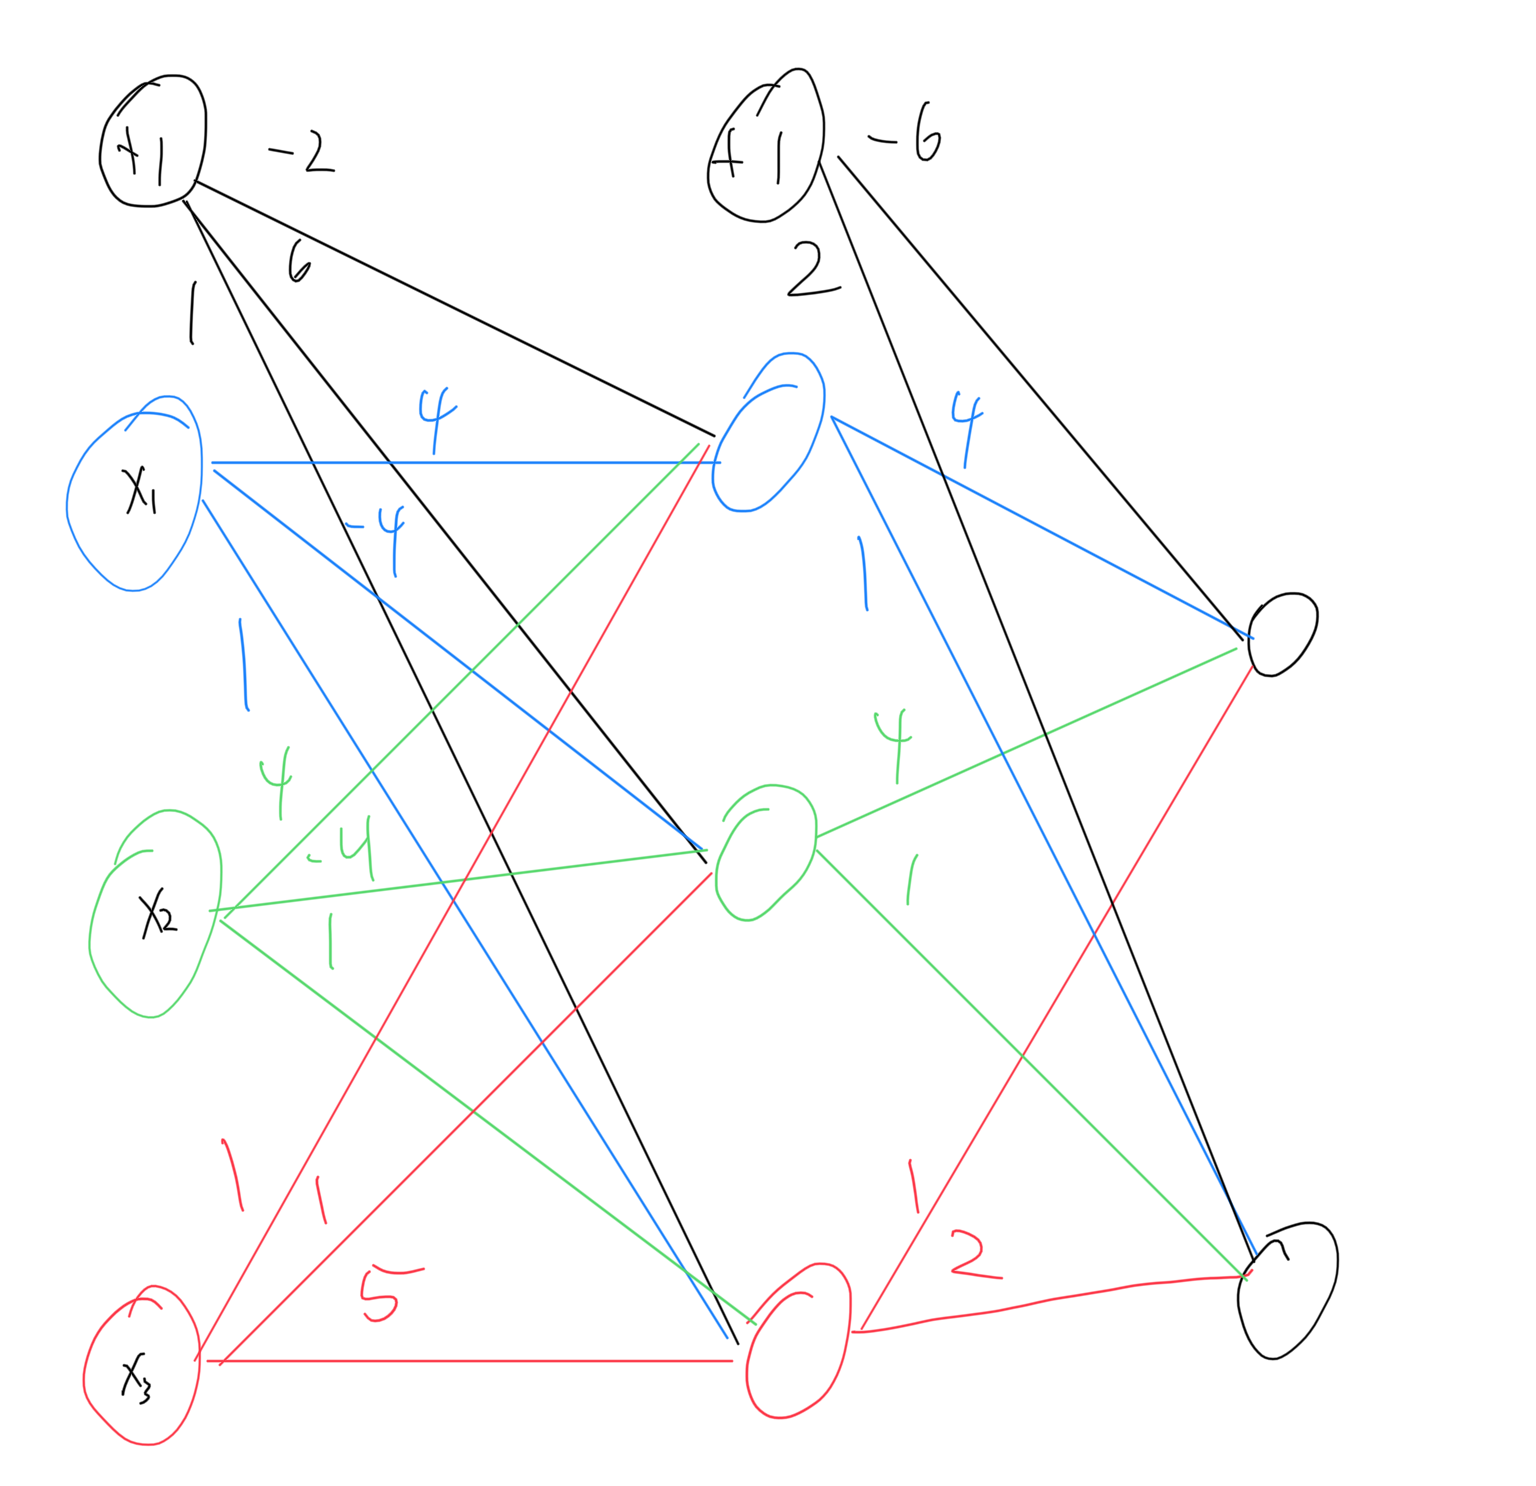
\includegraphics[height=\pdfpageheight*1/3]{images/1a.png}
		\caption{Drawing of Neural Network}
		\label{fig:1:a}
	\end{figure}
	
	\item 
	\[ z^{(i+1)} = W^{(i)}a^{(i)} + b^{(i)}, a^{(i)} = \sigma\left(z^{(i)}\right) \]
	The first $ a $ is $ x $.
	\[h_{W,b}(\mathbf{x}) = \sigma\left(W^{(2)}\sigma\left(W^{(1)}x + b^{(1)}\right)+b^{(2)}\right)\]
	\[ = 
	\sigma \left(
	\begin{bmatrix}
		4 & 4 & 1\\
		1 & 1 & 2
	\end{bmatrix}
	\sigma \left(
	\begin{bmatrix}
		4 & 4 & 1\\
		-4 & -4 & 1\\
		1 & 1 & -5
	\end{bmatrix}
	\begin{bmatrix}
		1\\
		2\\
		3
	\end{bmatrix} 
	+
	\begin{bmatrix}
		-2\\
		6\\
		1
	\end{bmatrix} \right)
+
	\begin{bmatrix}
	-6\\
	2
	\end{bmatrix} \right) \]
	\[ = \begin{bmatrix}
		0.1406\ldots\\
		0.9547\ldots
	\end{bmatrix}
	\]
	
	\item 
	\begin{itemize}
		\item $ \delta_{1}^{(3)} = \dfrac{\partial J}{\partial z_{1}^{(3)}} = -\left(y_1 - \sigma\left(z_{1}^{3}\right)\right)  \sigma^{\prime}\left(z_{1}^{3}\right) \approx -\left(1 - 0.1406\right) \left(0.1406* (1-0.1406)\right) \approx -0.1038$
		
		\item $ a_{1}^{(2)} = \sigma\left( 
			\begin{bmatrix}
				4 & 4 & 1\\
			\end{bmatrix} 
			\begin{bmatrix}
			1 & 2 & 3\\
			\end{bmatrix}
		^T 
		+ 
			\begin{bmatrix}
				-2\\
			\end{bmatrix}
		\right) \approx 0.9999$
		
		$ \dfrac{\partial J}{\partial W_{11}^{(2)}} = \delta_{1}^{(l+1)} a_{1}^{(2)} = -0.1038 * 0.9999 \approx -0.1038 $
		
		\item $ \delta_{1}^{(2)} \rightarrow  \sum_{i=1}^{s_{l+1}} \delta_{i}^{(l+1)} W_{ij}^{(l)} \sigma^{\prime}\left(z_{j}^{(l)}\right) = \sum_{i=1}^{2} \delta_{i}^{3}W_{i1}^{2}\sigma^{\prime}\left(z_{1}^{2}\right) = \delta_{1}^{3}W_{11}^{2}\sigma^{\prime}\left(z_{1}^{2}\right) + \delta_{2}^{3}W_{21}^{2}\sigma^{\prime}\left(z_{1}^{2}\right)$\par
		$ \delta _{1}^{3} = -0.1038 $\par
		$ W_{11}^2 = 4 $\par
		$ \sigma^\prime \left(z_1^2\right) =  \sigma^\prime \left(
			\begin{bmatrix}
				4 & 4 & 1\\
			\end{bmatrix}\begin{bmatrix}
				1 & 2 & 3\\
			\end{bmatrix}^T + 
			\begin{bmatrix}
				-2\\
			\end{bmatrix}\right) = \sigma^\prime \left(13\right) =  \sigma(13) * (1-\sigma(13)) \approx 0$\par
		$ \delta^3_2 = -\left(0-0.9547\right) \left(0.9547 * (1-0.9547)\right) \approx 0.0413$\par
		$ W_{21}^2 = 1 $\par
		$ \sigma^\prime\left(z^2_1\right) = \sigma^\prime \left(
			\begin{bmatrix}
				-4 & -4 & 1
			\end{bmatrix}
			\begin{bmatrix}
				1 & 2 & 3
			\end{bmatrix}^T
			+ 
			\begin{bmatrix}
				6
			\end{bmatrix}
		\right) = \sigma^\prime (-3) = 0.0474 * (1-0.0474) = 0.0452$\par
		$ \delta_1^{(2)} = (\ldots) * 0 + 0.0413 * 1 * 0.0452 = 0.0018 $
		
		\item $ a_1^1 = 1 $\par		
		$ \dfrac{\partial J}{\partial W_{11}^{(1)}} = \delta_1^{(1)} a_1^{1} = 0.0452 $
	\end{itemize}
\end{enumerate}
\newpage

\section{}
\begin{enumerate}
	\item 
	Forward propagation:
	\begin{align*}
		a^{(1)} &= (1,0)^T\\
		z^{(2)} &= 
		\begin{bmatrix}
			1 & 2\\
			3 & 4
		\end{bmatrix}
		\begin{bmatrix}
			1 \\
			0
		\end{bmatrix}
	+ 
		\begin{bmatrix}
			1\\
			-1
		\end{bmatrix}
	= 
		\begin{bmatrix}
			2\\
			2
		\end{bmatrix}\\
	a^{(2)} &= 
		\begin{bmatrix}
			0.8808\\
			0.8808
		\end{bmatrix}\\
	z^{(3)} &= 
		\begin{bmatrix}
			1 & 2
		\end{bmatrix}
		\begin{bmatrix}
			0.8808\\
			0.8808
		\end{bmatrix}
	+ 
		\begin{bmatrix}
			1
		\end{bmatrix}
	=
		\begin{bmatrix}
			3.64
		\end{bmatrix}\\
	a^{(3)} &= 	
		\begin{bmatrix}
			0.9745
		\end{bmatrix}
	\end{align*}
	Backward propagation:
	\begin{align*}
		\delta^{(3)} &= \dfrac{\partial J}{\partial b^{(2)}} = -\left(1 - 0.9745\right)0.9745 \left(1-0.9745\right) = [-0.000634]\\
		\delta^{(2)} &= \dfrac{\partial J}{\partial b^{(1)}} =
			\begin{bmatrix}
				\delta_1^{3} * W_{11}^{(2)} * \sigma^\prime\left(z_1^{(2)}\right)\\
				\delta_1^{(3)} * W_{12}^{(2)} * \sigma^\prime \left(z_2^{(2)}\right)
			\end{bmatrix}
		=
			\begin{bmatrix}
				-0.000634 * 1 * \left(0.8808 * (1-0.8808)\right)\\
				-0.000634 * 2 * \left(0.08808 * (1-0.8808)\right)
			\end{bmatrix}
		=
			\begin{bmatrix}
				-0.000067\\
				-0.00013
			\end{bmatrix}\\
		\dfrac{\partial J}{\partial W^{(2)}} &= 
			\begin{bmatrix}
				\delta_1^{(3)}a_1^{(2)} & \delta_1^{(3)}a_2^{(2)}\\
			\end{bmatrix}
		=	
			\begin{bmatrix}
				-0.00063 * 0.8808& -0.00063*0.8808
			\end{bmatrix}
		= \begin{bmatrix}
			-0.00055& -0.00055
		\end{bmatrix}\\
	\dfrac{\partial J}{\partial W^{(1)}} &= 
		\begin{bmatrix}
			\delta_1^{(2)} * a_1^{(1)} & \delta_1^{(2)} * a_2^{(1)}\\
			\delta_2^{(2)} * a_1^{(1)} & \delta_2^{(2)} * a_2^{(1)}
		\end{bmatrix}
	=
		\begin{bmatrix}
			-0.000067 * 1 & -0.000067 * 0\\
			-0.00013 * 1 & -0.00013 * 0
		\end{bmatrix}
	=
		\begin{bmatrix}
			-0.000067 & 0\\
			-0.00013 & 0
		\end{bmatrix}
	\end{align*}

	\item Forward propagation:
	\begin{align*}
		a^{(1)} &= (0,1)^T\\
		z^{(2)} &= 
			\begin{bmatrix}
				1 & 2\\
				3 & 4
			\end{bmatrix}
			\begin{bmatrix}
				0\\
				1
			\end{bmatrix}
		+
			\begin{bmatrix}
				1\\
				-1
			\end{bmatrix}
		=
			\begin{bmatrix}
				3\\
				3
			\end{bmatrix}\\
		a^{(2)} &= 
			\begin{bmatrix}
				.9525\\
				.9525
			\end{bmatrix}\\
		z^{(3)} &= 
			\begin{bmatrix}
				1 & 2
			\end{bmatrix}
			\begin{bmatrix}
				.9525\\
				.9525
			\end{bmatrix}
		+
			\begin{bmatrix}
				1
			\end{bmatrix}
		= 	
			\begin{bmatrix}
				3.8575
			\end{bmatrix}\\
		a^{(3)} &=
			\begin{bmatrix}
				.9793
			\end{bmatrix}
	\end{align*}
	Backward Propagation:
	\begin{align*}
		\delta^{(3)} &= \dfrac{\partial J}{\partial b^{(2)}} = 
			-\left(0 - a^{(3)}\right)\left(a^{(3)}\left(1-a^{(3)}\right)\right) = [0.01985]\\
		\delta^{(2)} &= \dfrac{\partial J}{\partial b^{(1)}} = 
			\begin{bmatrix}
				\delta^{(3)} W_{11}^{(2)} \sigma^\prime \left(z_1^{(2)}\right)\\
				\delta^{(3)} W_{12}^{(2)} \sigma^\prime \left(z_2^{(2)}\right)
			\end{bmatrix}
			=
			\begin{bmatrix}
				0.01985*1*0.9525*(1-0.9525)\\
				0.01985*2*0.09525*(1-0.9525)
			\end{bmatrix}
			=
			\begin{bmatrix}
				0.000898\\
				0.001796
			\end{bmatrix}\\
		\dfrac{\partial J}{\partial W^{(2)}} &=
			\begin{bmatrix}
				\delta^{(3)} * a_1^{(2)} & \delta^{(3)}*a_2^{(2)}
			\end{bmatrix}
			=
			\begin{bmatrix}
				0.01985 * 0.9525 & 0.01985 * 0.09525
			\end{bmatrix}
			=
			\begin{bmatrix}
				0.01891 & 0.01891
			\end{bmatrix}\\
		\dfrac{\partial J}{\partial W^{(1)}} &= 
			\begin{bmatrix}
				\delta_1^{(2)} * a_1^{(1)} & \delta_1^{(2)} * a_2^{(1)}\\
				\delta_2^{(2)} * a_1^{(1)} & \delta_2^{(2)} * a_2^{(1)}
			\end{bmatrix}
			=
			\begin{bmatrix}
				0.000898 * 0 & 0.000898 * 1\\
				0.001796 * 0 & 0.001796*1
			\end{bmatrix}
			=
			\begin{bmatrix}
				0 & 0.000898\\
				0 & 0.001796
			\end{bmatrix}
	\end{align*}

	\item [\textbf{Update}] To do the update step, we just average the respective terms, multiply by the learning rate, and subtract.
	\begin{align*}
		W^{(1)} &= W^{(1)} - \dfrac{\alpha}{2} \left(
			\begin{bmatrix}
				-0.000067 & 0\\
				-0.00013 & 0
			\end{bmatrix}
			+
			\begin{bmatrix}
				0 & 0.000898\\
				0 & 0.001796
			\end{bmatrix}
			\right)\\
		&= 
			\begin{bmatrix}
				1 & 2\\
				3 & 4
			\end{bmatrix}
			- \dfrac{0.2}{2}
			\begin{bmatrix}
				-0.000067 & 0.000898\\
				-0.00013 & 0.001796
			\end{bmatrix}\\
		&=
			\begin{bmatrix}
				1.00001 & 1.99991\\
				3.00001 & 3.99982
			\end{bmatrix}
	\end{align*}
	\begin{align*}
		b^{(1)} &= b^{(1)} - \dfrac{\alpha}{2}\left(
			\begin{bmatrix}
			-0.000067\\
			-0.00013
			\end{bmatrix}
			+
			\begin{bmatrix}
				0.000898\\
				0.001796
			\end{bmatrix}
			\right)\\
		&= 
			\begin{bmatrix}
				1\\
				-1
			\end{bmatrix}
			- \dfrac{0.2}{2}
			\begin{bmatrix}
				0.000831\\
				0.001666
			\end{bmatrix}\\
		&= 
			\begin{bmatrix}
				0.999917\\
				-1.00017
			\end{bmatrix}
	\end{align*}
	\begin{align*}
		W^{(2)} &= W^{(2)} - \dfrac{\alpha}{2}\left(
			\begin{bmatrix}
				-0.00055 & -0.00055
			\end{bmatrix}
			+
			\begin{bmatrix}
				0.01891 & 0.01891
			\end{bmatrix}
			\right)\\
		&= 
			\begin{bmatrix}
				1 & 2
			\end{bmatrix}
			- \dfrac{0.2}{2}
			\begin{bmatrix}
				0.01836 & 0.01836
			\end{bmatrix}\\
		&= 
			\begin{bmatrix}
				0.99814 & 1.99814
			\end{bmatrix}
	\end{align*}
	\begin{align*}
		b^{(2)} &= b^{(2)} - \dfrac{\alpha}{2}\left([-0.000634]+[0.01985]\right)\\
		&= [1] - \dfrac{0.2}{2}\left(0.019216[]\right)\\
		&= [0.980784]
	\end{align*}
\end{enumerate}
\newpage

\section*{4}
Overfitting will be a problem for small training sets and models with a large number of parameters.
\newpage

\section*{7}
\begin{enumerate}[(a)]
	\item \,
		\begin{figure}[H]
			\centering
			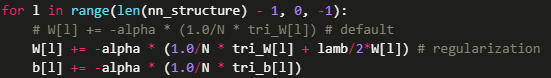
\includegraphics[width=\textwidth/2]{images/7achange.png}
			\caption{Changes for regularization}
			\label{fig:7:a:change}
		\end{figure}
		I also added lamb as an argument, of course.
		\begin{figure}[H]
			\centering
			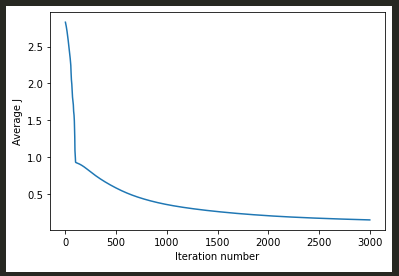
\includegraphics[width=\textwidth/2]{images/7agraph.png}
			\caption{Error v. Iteration}
			\label{fig:7:a:J}
		\end{figure}
		The accuracy was 94.297\% when lamb=1.
	
	\item \,
		\begin{figure}[H]
			\centering
			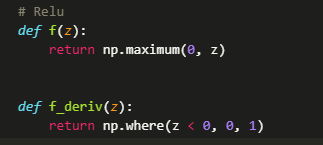
\includegraphics[width=\textwidth/2]{images/7bchange.png}
			\caption{Changes for ReLu}
			\label{fig:7:b:change}
		\end{figure}
		\begin{figure}[H]
			\centering
			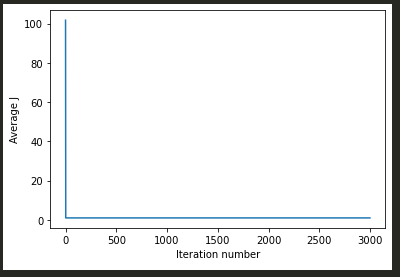
\includegraphics[height=\textwidth/2]{images/7bgraph.png}
			\caption{Error v. Iteration}
			\label{fig:7:b:J}
		\end{figure}
		The accuracy with the ReLu function was 9.75\%.
		
	\item \,
		\begin{figure}[H]
			\centering
			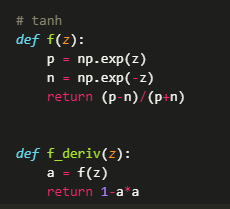
\includegraphics[width=\textwidth/2]{images/7cchange.png}
			\caption{Changes for tanh}
			\label{fig:7:c:changes}
		\end{figure}
		\begin{figure}[H]
			\centering
			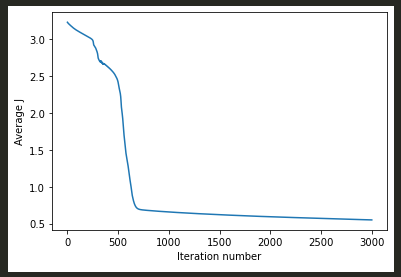
\includegraphics[width=\textwidth/2]{images/7cgraph.png}
			\caption{Error v. Iteration}
			\label{fig:7:c:graph}
		\end{figure}
		The accuracy with the tanh function was 88.873\%.
		
	\item ELU results in overflow. 
		\begin{figure}[H]
			\centering
			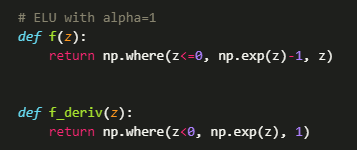
\includegraphics[width=\textwidth/2]{images/7dchange.png}
			\caption{Changes}
			\label{fig:7:d:changes}
		\end{figure}
		\begin{figure}[H]
			\centering
			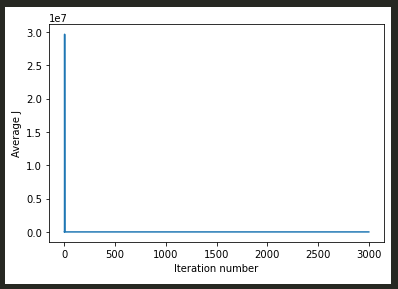
\includegraphics[width=\textwidth/2]{images/7dgraph.png}
			\caption{Error v. Iteration}
			\label{fig:7:d:graph}
		\end{figure}
		The accuracy with the ELU function (with overflow) was 9.04\%.
	
	\item \,
		\begin{figure}[H]
			\centering
			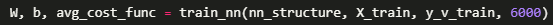
\includegraphics[width=\textwidth/2]{images/7echange.png}
			\caption{Changes}
			\label{fig:7:e:change}
		\end{figure}
		\begin{figure}[H]
			\centering
			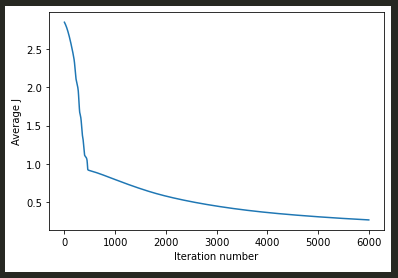
\includegraphics[width=\textwidth/2]{images/7egraph.png}
			\caption{Erorr v. Iteration}
			\label{fig:7:e:graph}
		\end{figure}
		Increasing the iterations to 6000 resulted in an accuracy of 92\%.
		
	\item \,
		\begin{figure}[H]
			\centering
			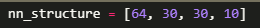
\includegraphics[width=\textwidth/2]{images/7fchange.png}
			\caption{Changes}
			\label{fig:7:f:change}
		\end{figure}
		\begin{figure}[H]
			\centering
			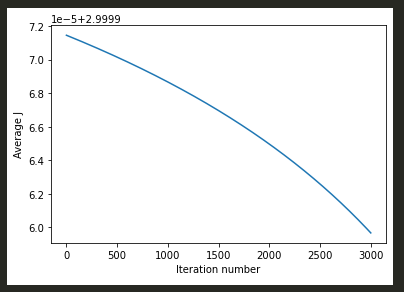
\includegraphics[width=\textwidth/2]{images/7fgraph.png}
			\caption{Error v. Iteration}
			\label{fig:7:f:graph}
		\end{figure}
		\begin{figure}[H]
			\centering
			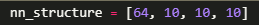
\includegraphics[width=\textwidth/2]{images/7fchange1.png}
			\caption{Changes}
			\label{fig:7:f:change}
		\end{figure}
		\begin{figure}[H]
			\centering
			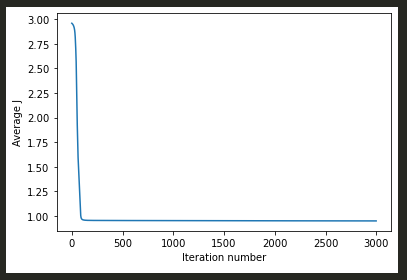
\includegraphics[width=\textwidth/2]{images/7fgraph1.png}
			\caption{Error v. Iteration}
			\label{fig:7:f:graph}
		\end{figure}
		Neither of the hidden layer changes had high accuracy: 5\% and 9.3\%, respectively. 
	
\end{enumerate}
The highest accuracy of 94 \% came from regularization with lamb=1.



\end{document}